\documentclass[tikz, border=2pt]{standalone}

\usepackage{amsmath,amssymb}
\usepackage{pgfplots}
\pgfplotsset{compat=1.18}
\usepgfplotslibrary{groupplots}
\usetikzlibrary{arrows.meta}
\usepackage{xcolor}

\definecolor{utnblue}{RGB}{0, 51, 102}

\begin{document}
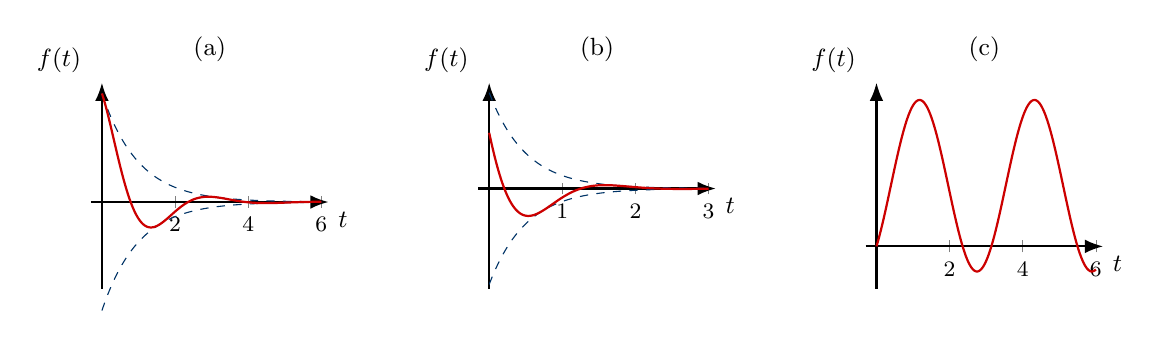
\begin{tikzpicture}[>=Latex, font=\small]

\pgfplotsset{
  every axis/.append style={
    axis lines=middle,
    axis line style={->, thick, black},
    width=4.6cm, height=4.2cm,
    xlabel={$t$}, ylabel={$f(t)$},
    xlabel style={anchor=north west},
    ylabel style={rotate=0, anchor=south east, at={(axis description cs:0,1)}},
    ytick=\empty,
    xticklabel style={font=\footnotesize},
    title style={yshift=-2pt},
    samples=200,
    clip=false,
  },
  resp/.style={red!80!black, thick},
  env/.style={utnblue, thin, dashed},
}

\begin{groupplot}[
  group style={group size=3 by 1, horizontal sep=1.9cm},
]
  % ===== (a) coseno amortiguado: 3 e^{-t} cos(2t) =====
  \nextgroupplot[domain=0:6, xmin=-0.3, xmax=6.2, ymin=-2.4, ymax=3.3, title={(a)}]
    \addplot[env] {3*exp(-x)};
    \addplot[env] {-3*exp(-x)};
    \addplot[resp] {3*exp(-x)*cos(deg(2*x))};

  % ===== (b) coseno+seno amortiguados: e^{-2t}[5cos(3t) - 7sin(3t)] =====
  \nextgroupplot[domain=0:3, xmin=-0.15, xmax=3.1, ymin=-9, ymax=9.5, title={(b)}]
    \addplot[env] {sqrt(74)*exp(-2*x)};
    \addplot[env] {-sqrt(74)*exp(-2*x)};
    \addplot[resp] {exp(-2*x)*(5*cos(deg(3*x)) - 7*sin(deg(3*x)))};

  % ===== (c) oscilacion sostenida: (1/2)[1 - cos 2t + sin 2t] =====
  \nextgroupplot[domain=0:6, xmin=-0.3, xmax=6.2, ymin=-0.35, ymax=1.35, title={(c)}]
    \addplot[resp] {0.5 - 0.5*cos(deg(2*x)) + 0.5*sin(deg(2*x))};
\end{groupplot}
\end{tikzpicture}
\end{document}
